%%%%%%%%%%%%%%%%%%%%%%% CHAPTER - 4 %%%%%%%%%%%%%%%%%%%%\\
\chapter{Results and Discussion}
\label{C4} %%%%%%%%%%%%%%%%%%%%%%%%%%%%

%\noindent\rule{\linewidth}{2pt}
%%%%%%%%%%%%%%%%%%%%%%%%%%%%%%%%%%%%%%%%%%%%%%%%%%%%%%%%%%%%%%%%%%%%%%%%%%%%%%%%%%
\par
Various types of vector embeddings were used in this evaluation process to determine the best possible way for marking. The experiments are elaborated below. \\
\par
In Natural Language Processing, words or collections of words are represented by vectors to make sense to the computer. There are various techniques for creating these embeddings like, \textit{Word2Vec, Doc2Vec, Bert,} etc. \\
\par
\textbf{BERT} \textit{(Bidirectional Encoder Representations from Transformers)} is a comparatively newer NLP model developed by Google researchers. It uses transformers which have two main mechanisms, encoding and decoding. It learns relationships between words from a huge corpus of data. In our project, we pre-trained base Bert model and SciBert(Bert model trained on a huge corpus of scientific writings). Bert model can also be used to generate sentence embeddings. The embeddings are then used to calculate similarity. This was done with both aforementioned models of Bert but the result was not satisfactory. The dataset contained a range of answers, some good and some bad, but the cosine similarity from Bert gave a similarity range between 80-90\% (80\% for base pre-trained Bert and minimum 83\% for SciBert). \\
\par
\textbf{Word2Vec} is one of the famous word embedding techniques in the field of Natural language Processing. It uses a neural network to generate a vector space of a certain dimension, where each word is represented by a vector in the space. In the vector space, words used in similar contexts are closer than other words. Also, the semantic meaning is preserved in the model. As a famous example, in a well-trained model, if one subtracts the vector ‘man’ from that of ‘king’ and adds the vector of ‘woman’, the resultant vector should represent ‘queen’. \textbf{WMD or Word Mover’s Distance} \textit{(NLP implementation of Earth Mover’s Distance)} can be used to calculate the distance between two sentences efficiently but in the context of evaluating answers of multiple lines where even the number of lines, therefore number of words, can differ from person to person. Moreover, it is hard to map distance with similarity. For these reasons, Word2Vec was not used in this evaluation approach. \\
\par
Instead, we use \textbf{Doc2Vec}, an implementation of the previously mentioned Word2vec model. In Doc2Vec, instead of word embeddings, document embedding is used. Doc2Vec captures what kind of words are normally used together and determines vectors for each document(here, answer script). As Doc2Vec is an implementation of Word2Vec, it also has two variances. One is a \textbf{Paragraph Vector With A Distributed Bag Of Words} \textit{(PVDBOW)}, parallel to a Continuous Bag Of Words(CBOW) in Word2Vec and a \textbf{Distributed Memory Model Of Paragraph Vectors} \textit{(PV-DM)}, similar to skip-gram in Word2Vec. Here, PV-DM is used because of the small size of the dataset. As Doc2Vec determines a vector for each answer document, we can use \textbf{Cosine Similarity} to determine the similarity between an answer script and the ideal answer script for a certain question. Cosine Similarity is the cosine value of the angle between two vectors. It is an implementation of the concept of vector dot product. The formula for Cosine Similarity is given by
\par
\begin{equation}
    \boxed{\cos{\theta} $=$ \frac{\Vec{A} \cdot \Vec{B}}{\left | \Vec{A}\right |  \left | \Vec{B}\right |}}
\end{equation}
\par
where A and B are two vectors. The value of Cosine Similarity ranges between -1 and 1. Values near 1 mean they are the same in meaning, and 0 means they have little to no similarity. Values near -1 mean they have opposite meanings. For the Data Mining Dataset, a Doc2Vec model with a dimension of 100 is trained after preprocessing. After training the Doc2Vec model, the answer scripts are clustered.
There exist many different kinds of clustering algorithms, like K-means, K-medians, DBSCAN, etc. If we know the number of clusters, K-means is a good choice, but in this context, the number of clusters cannot be determined beforehand without trial and error. This can be countered with the DBSCAN clustering algorithm because it works in the general case. The DBSCAN algorithm has two hyperparameters, eps which is the radius of the neighborhood of a certain point, and MinPts which is the minimum number of necessary points in eps radius to make a cluster. MinPts is taken as 3 to maximize the number of possible clusters, the value of eps is calculated from plotted graphs as they vary from question to question. The graphs are depicted below. \\

% Image 1a
\begin{figure}[H]
    \centering
    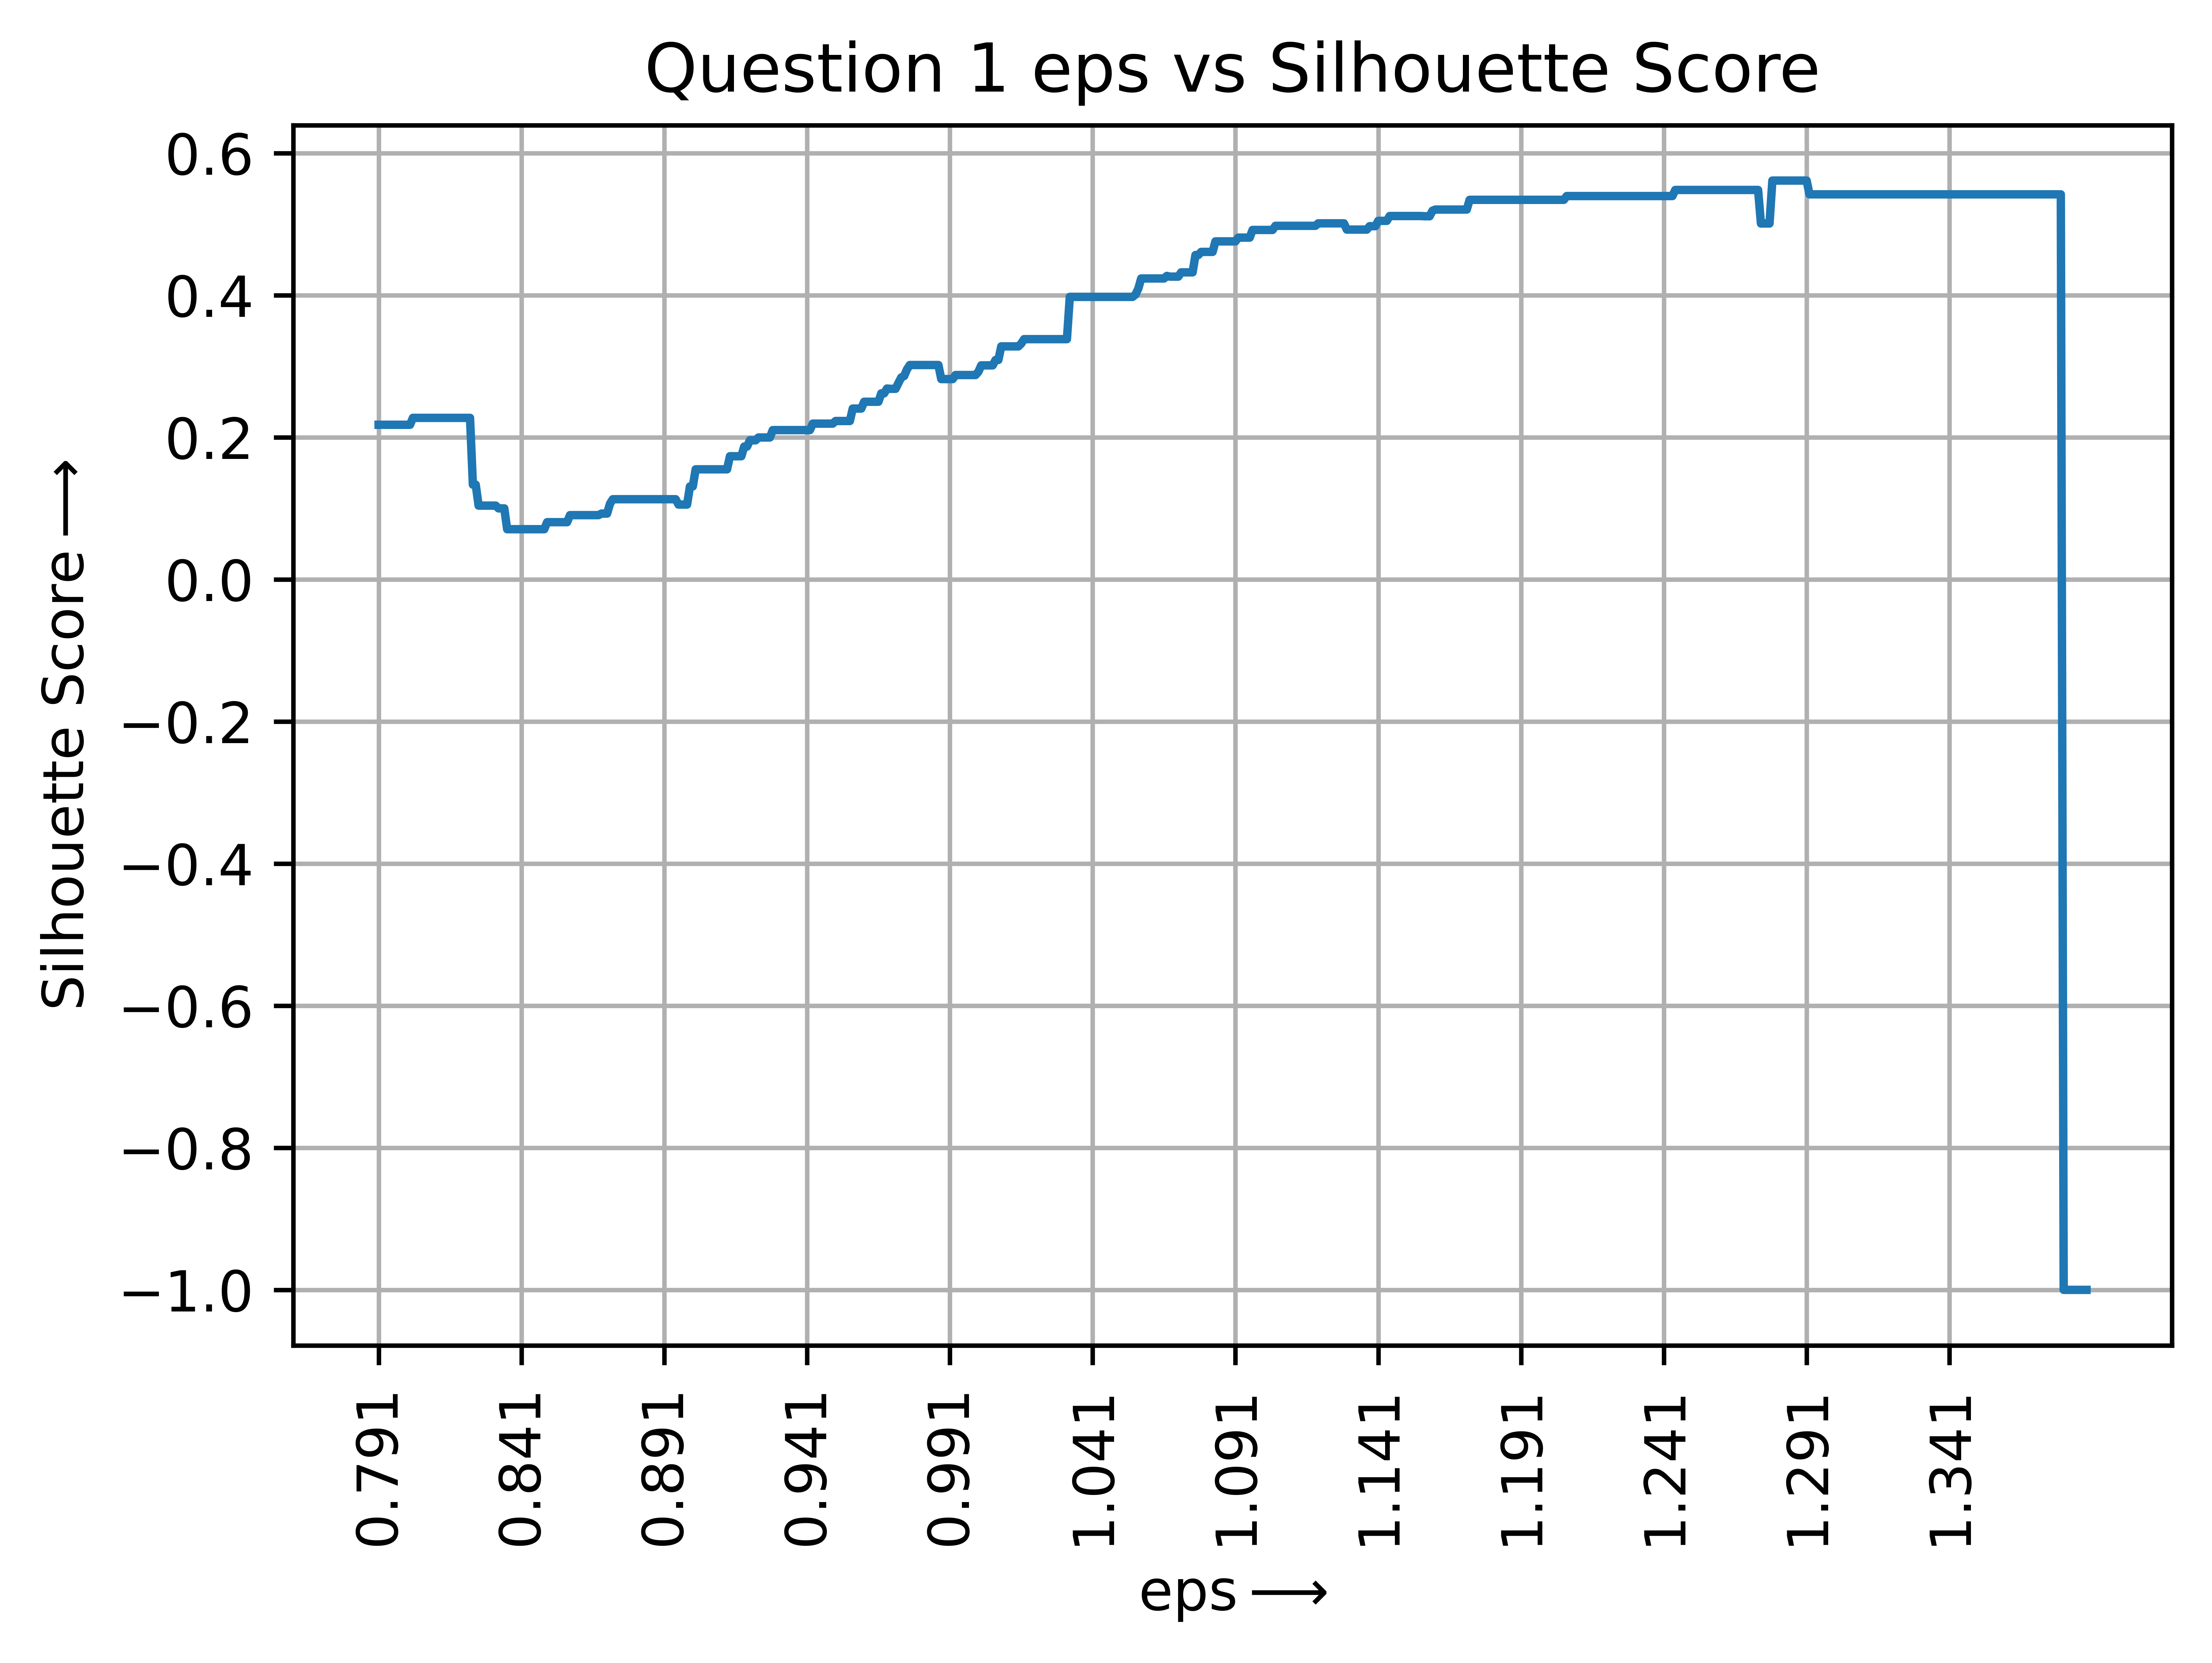
\includegraphics[width=0.75\linewidth]{IMAGE/eps&Silhouette.png}
    \caption{Question 1 eps vs Silhouette Score}
    \label{fig11}
\end{figure}

% Image 2a
\begin{figure}[H]
    \centering
    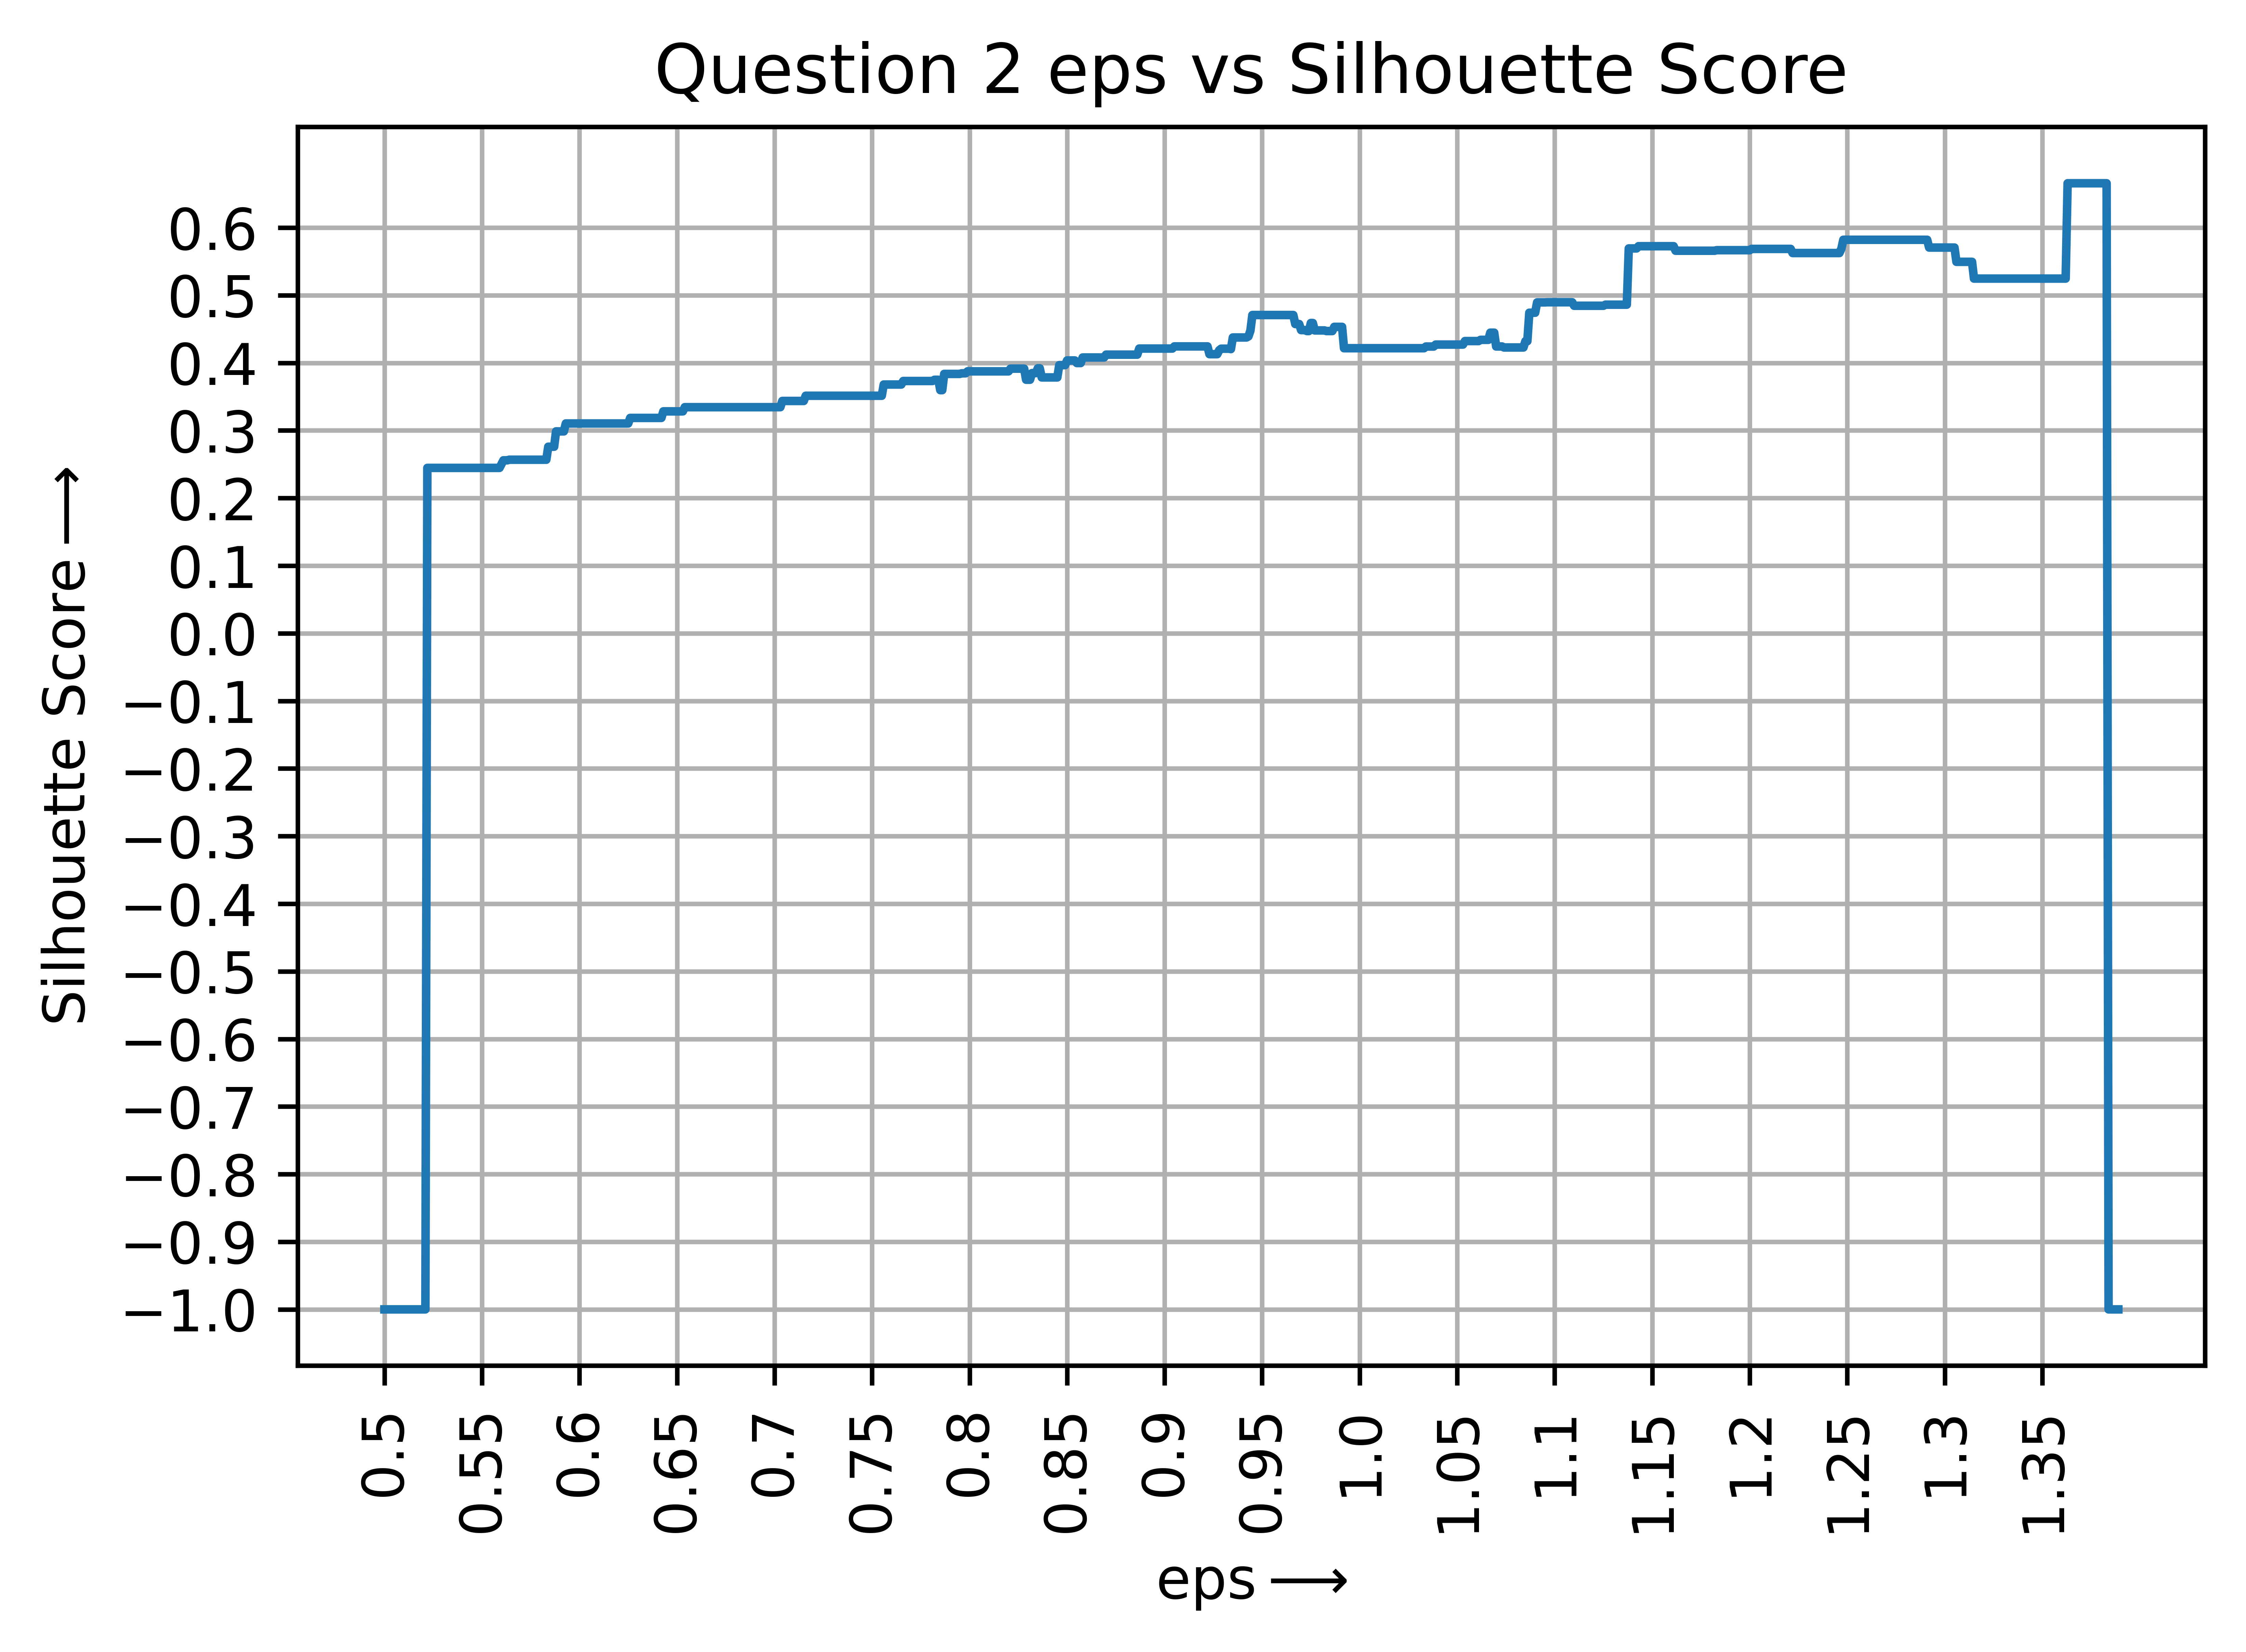
\includegraphics[width=0.75\linewidth]{IMAGE/q2_eps&Silhouette.png}
    \caption{Question 2 eps vs Silhouette Score}
    \label{fig12}
\end{figure}

% Image 3a
\begin{figure}[H]
    \centering
    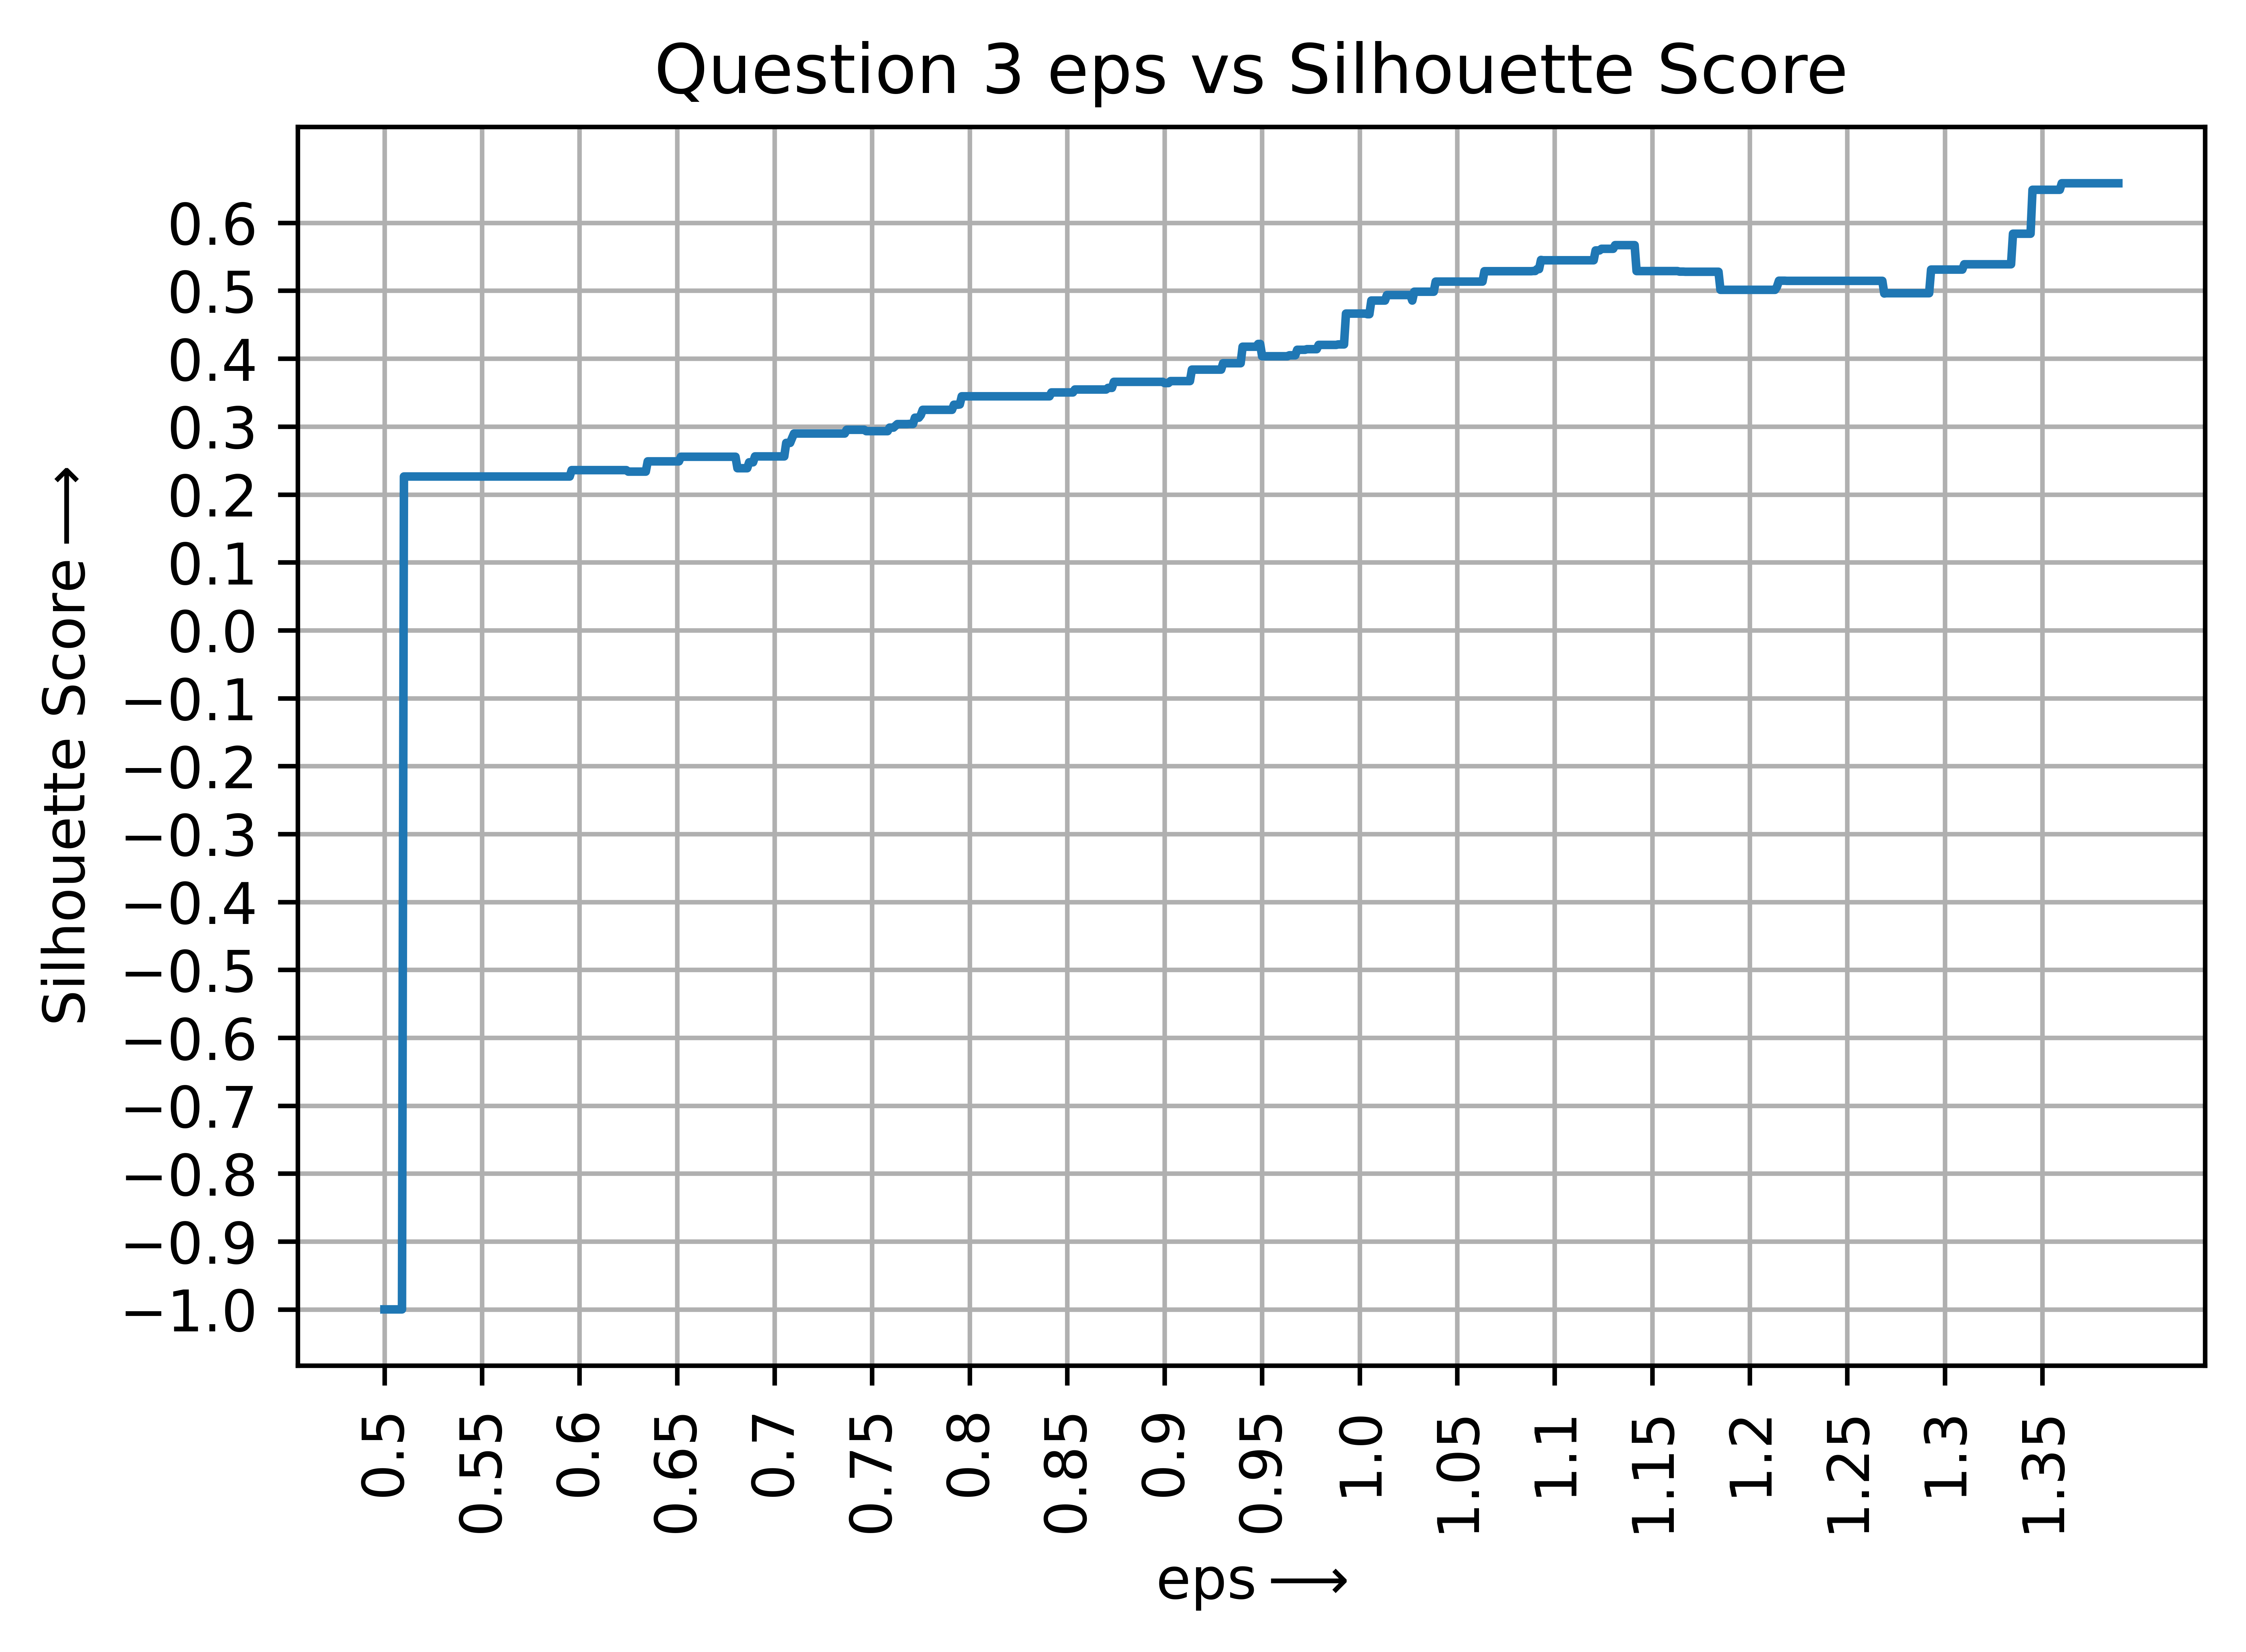
\includegraphics[width=0.75\linewidth]{IMAGE/q3_eps&Silhouette.png}
    \caption{Question 3 eps vs Silhouette Score}
    \label{fig13}
\end{figure}

% Image 4a
\begin{figure}[H]
    \centering
    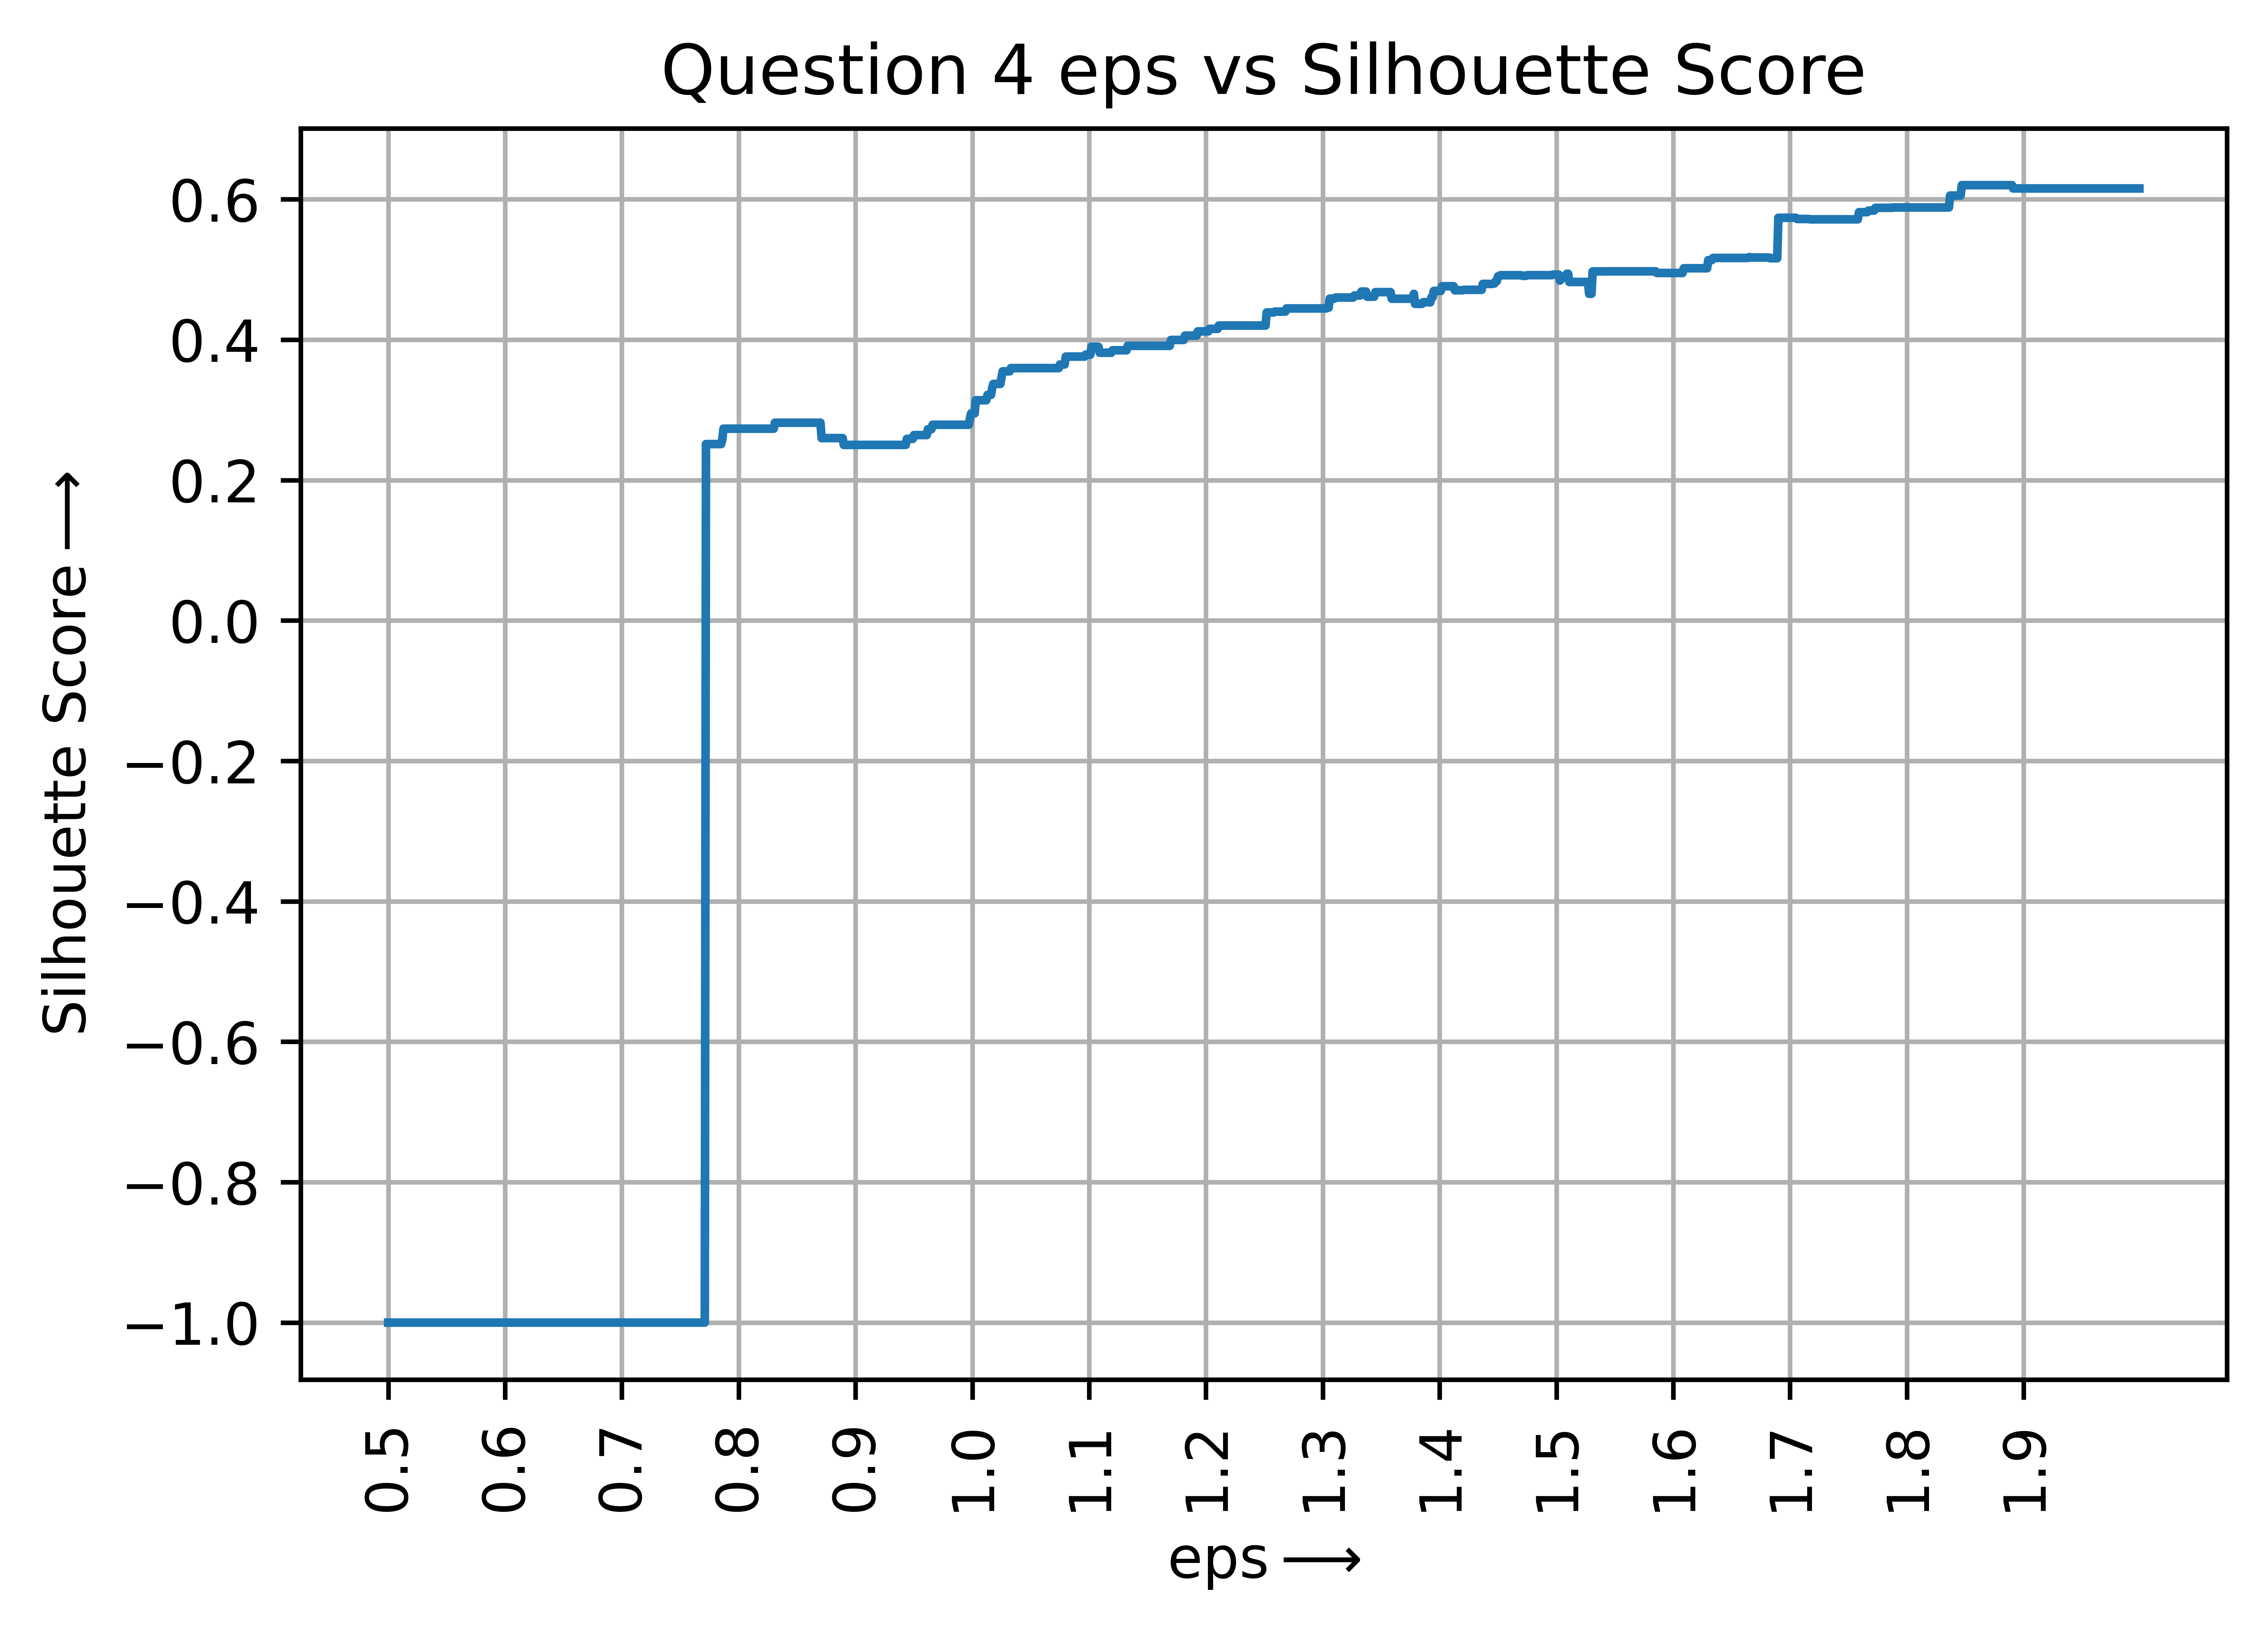
\includegraphics[width=0.75\linewidth]{IMAGE/q4_eps&Silhouette.png}
    \caption{Question 4 eps vs Silhouette Score}
    \label{fig14}
\end{figure}

% Image 5a
\begin{figure}[H]
    \centering
    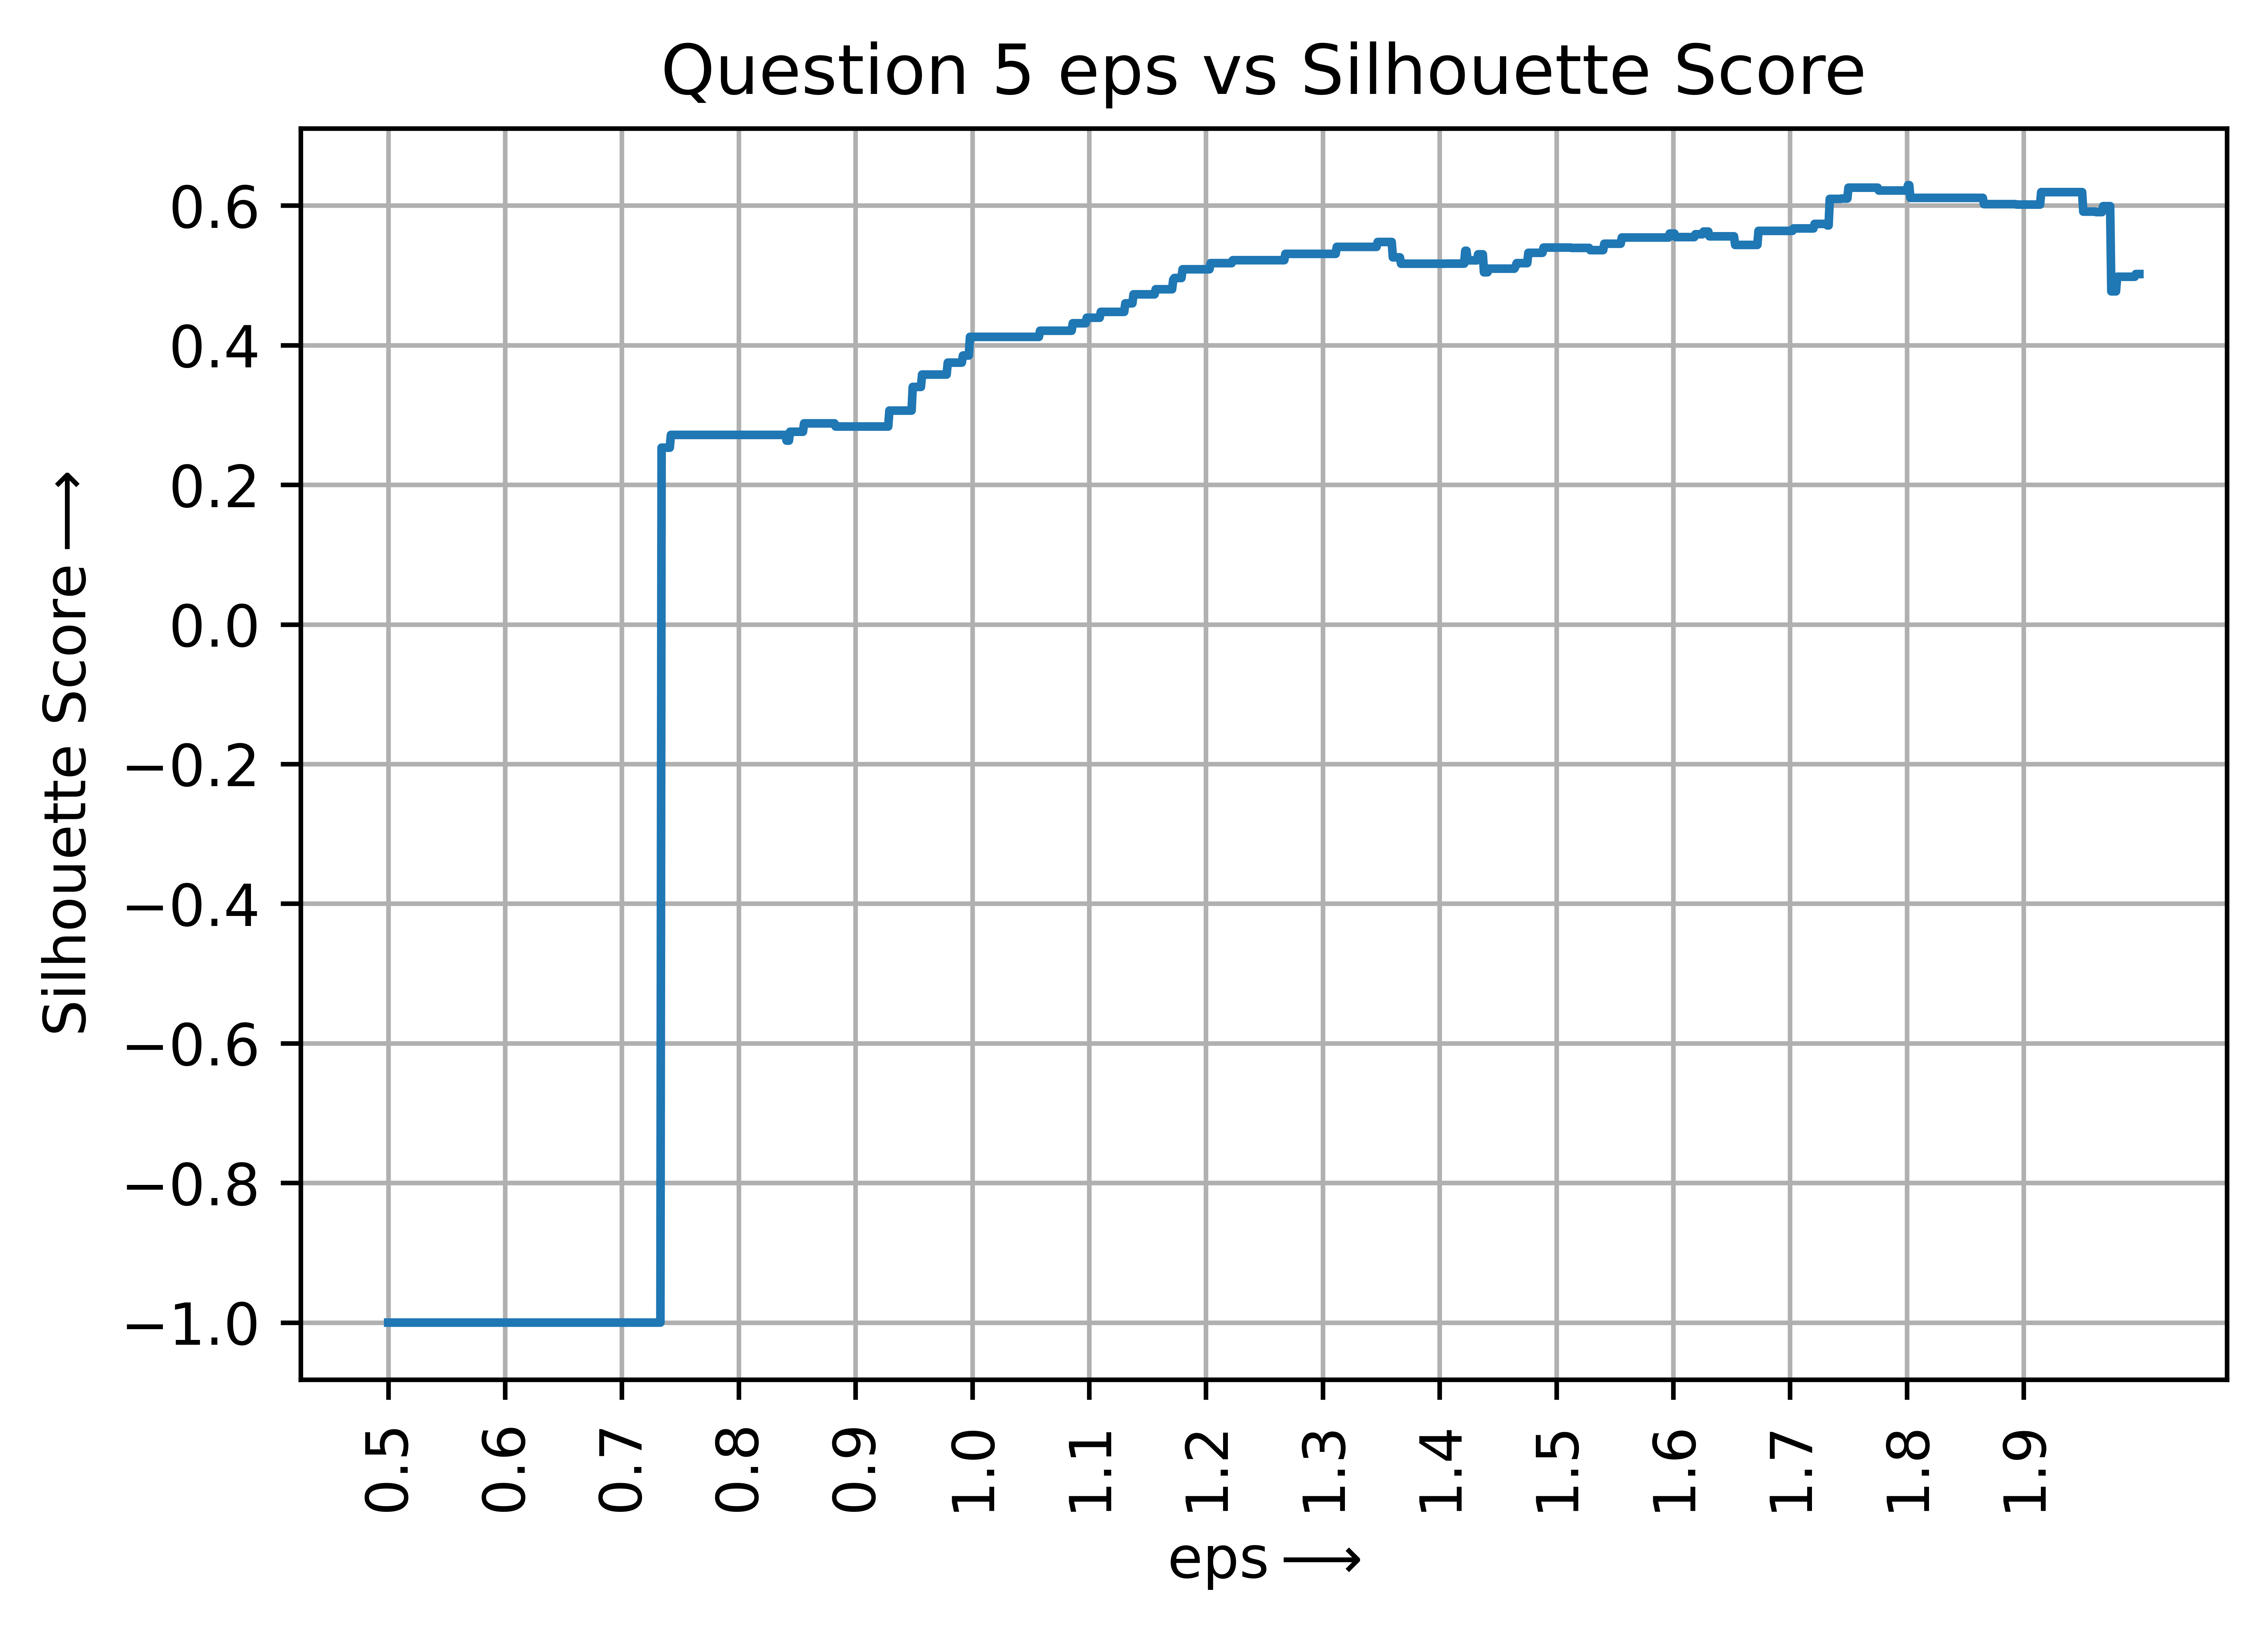
\includegraphics[width=0.75\linewidth]{IMAGE/q5_eps&Silhouette.png}
    \caption{Question 5 eps vs Silhouette Score}
    \label{fig15}
\end{figure}
Silhouette score is steadily increasing with increasing EPS value, but there is a sudden dip. This is because the Silhouette score cannot be calculated when the number of clusters is 0 or 1, so those cases are explicitly handled and the score is made -1.

%%%%%%%%%%%%%%%%%%%%%%%%%%%%%%%%%%%%%%%%%%%%%%%%%%%%%%%%%%%%%%%%%%%%%%%%%%%%%%%%%%
% image 1b
\begin{figure}[H]
    \centering
    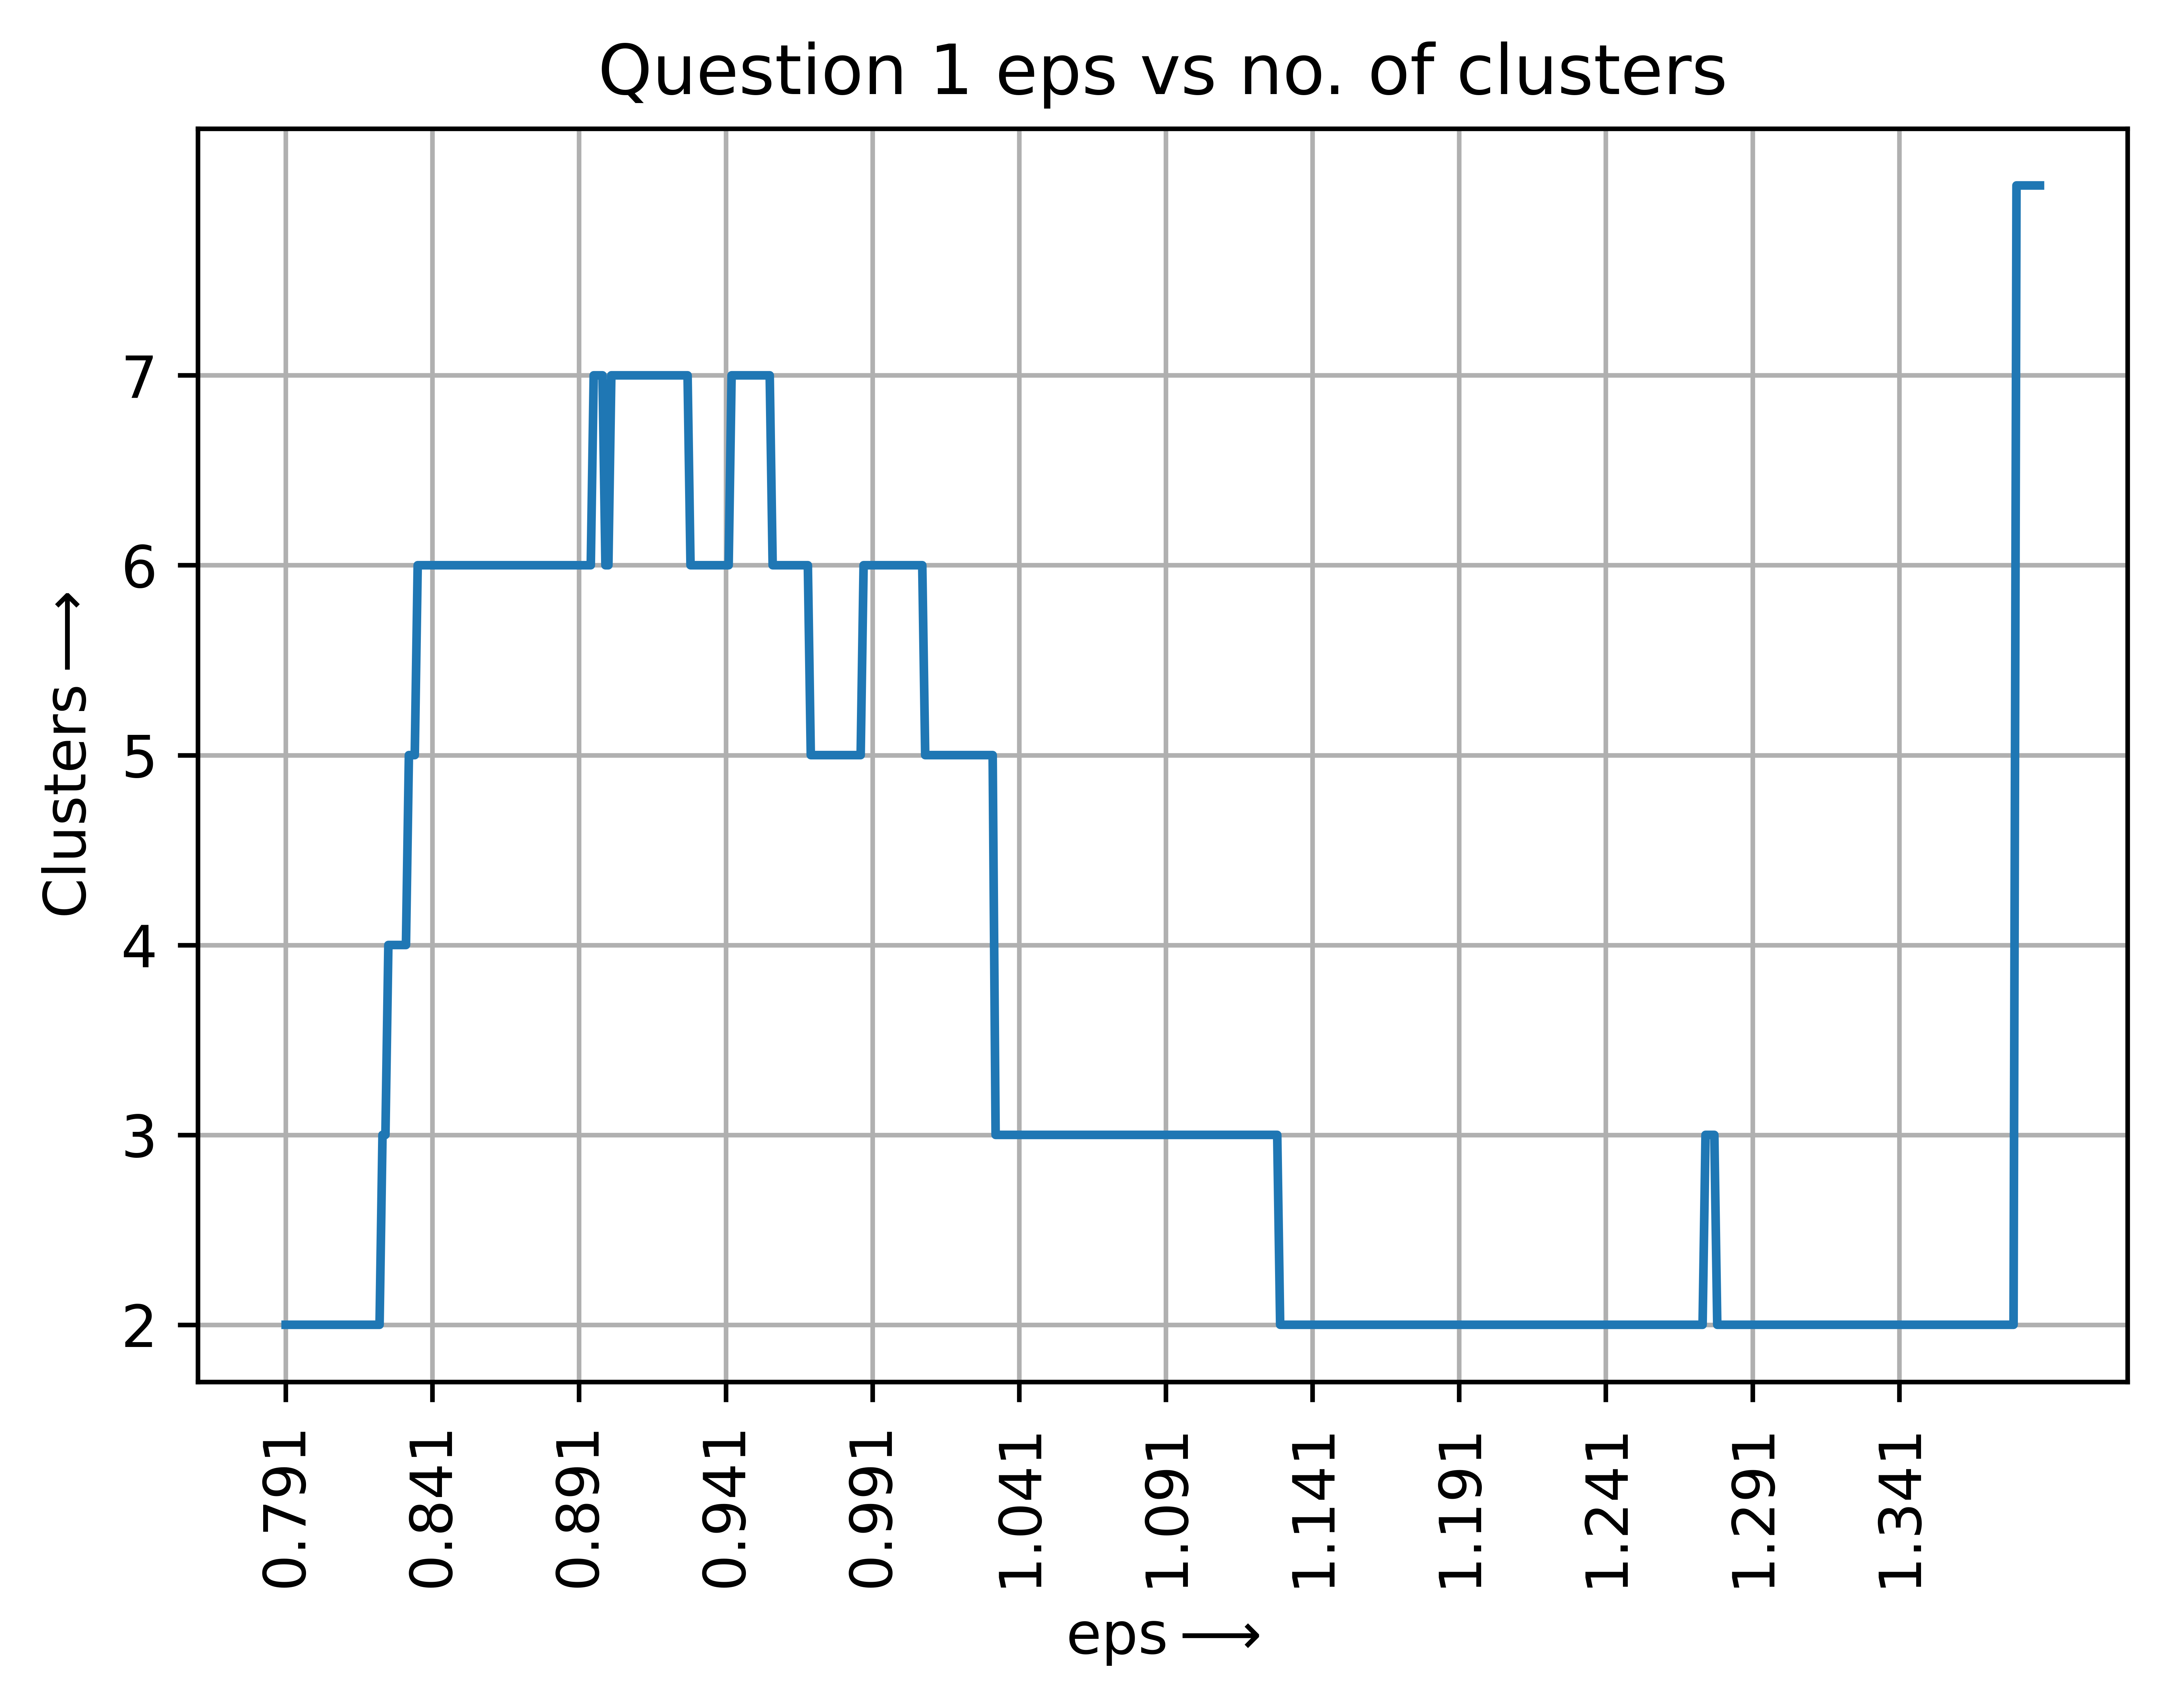
\includegraphics[width=0.75\linewidth]{IMAGE/eps&clusters.png}
    \caption{Question 1 eps vs Number of Clusters}
    \label{fig21}
\end{figure}

% image 2b
\begin{figure}[H]
    \centering
    \includegraphics[width=0.75\linewidth]{IMAGE/q2_eps&clusters.png}
    \caption{Question 2 eps vs Number of Clusters}
    \label{fig22}
\end{figure}

% image 3b
\begin{figure}[H]
    \centering
    \includegraphics[width=0.75\linewidth]{IMAGE/q3_eps&clusters.png}
    \caption{Question 3 eps vs Number of Clusters}
    \label{fig23}
\end{figure}

% image 4b
\begin{figure}[H]
    \centering
    \includegraphics[width=0.75\linewidth]{IMAGE/q4_eps&clusters.png}
    \caption{Question 4 eps vs Number of Clusters}
    \label{fig24}
\end{figure}

% image 5b
\begin{figure}[H]
    \centering
    \includegraphics[width=0.75\linewidth]{IMAGE/q5_eps&clusters.png}
    \caption{Question 5 eps vs Number of Clusters}
    \label{fig25}
\end{figure}

From the graph \ref{fig11}, it is observed that the value of eps is optimal in the range 0.841-0.991.\\

After clustering with optimal cluster count and Silhouette Score, marks are assigned to each cluster. The scripts not belonging to any clusters (Outliers), are handled separately. 

% Image m1
\begin{figure}[H]
    \centering
    \includegraphics[width=1\linewidth]{IMAGE/Marking.png}
    \caption{Question 1 Original vs Predicted Marking}
    \label{fig31}
\end{figure}

%%%%%%%%%%%%%%%%%%%%%%%%%%%%%%%%%%%%%%%%%%%%%%%%%%%%%%%%%%%%%%%%%%%%%%%%%%%%%%%%%%

% Image m1
\begin{figure}[H]
    \centering
    \includegraphics[width=1\linewidth]{IMAGE/Marking.png}
    \caption{Question 1 Original vs Predicted Marking}
    \label{fig31}
\end{figure}

% Image m2
\begin{figure}[H]
    \centering
    \includegraphics[width=1\linewidth]{IMAGE/q2_Marking.png}
    \caption{Question 2 Original vs Predicted Marking}
    \label{fig32}
\end{figure}

% Image m3
\begin{figure}[H]
    \centering
    \includegraphics[width=1\linewidth]{IMAGE/q3_Marking.png}
    \caption{Question 3 Original vs Predicted Marking}
    \label{fig33}
\end{figure}

% Image m4
\begin{figure}[H]
    \centering
    \includegraphics[width=1\linewidth]{IMAGE/q4_Marking.png}
    \caption{Question 4 Original vs Predicted Marking}
    \label{fig34}
\end{figure}

% Image m5
\begin{figure}[H]
    \centering
    \includegraphics[width=1\linewidth]{IMAGE/q5_Marking.png}
    \caption{Question 5 Original vs Predicted Marking}
    \label{fig35}
\end{figure}

In this approach, 5 different questions are considered for evaluation. The above graph is the depiction of a comparison between original marking by teachers and marks prediction by our model. There were 105 different answers for question number 1, and they are plotted serially. The quality of answers ranged from bad to good, and predicted marks were also similar with some rare exceptions. \\

This scheme rarely outputs low marks. Generally marking is done with a gap of 0.5, for example, in a question of full marks 3 (just like the graph above), the possible marks are 0, 0.5, 1, 1.5, 2, 2.5, and 3. But in the case of marking by a computer program, the possibilities are virtually endless. That is why there are many fluctuations in the predicted graph compared to the original marks. But the overall flow of the graph is very similar. We calculated the mean squared error by subtracting the original marks from the predicted marks, squaring it, adding this value for each answer script, and dividing it by the number of scripts. 
The calculated Mean Squared Error for question 1 to 5 are 0.07454, 0.10898, 0.17020, 0.18935 and 0.13414 respectively, which can be considered as a good score.
